\chapter{基于增量式集束调整的高效状态估计}\label{ch:ba}

iSAM2算法\cite{kaess2008isam,kaess2012isam2}创新性地在SLAM问题中使用了贝叶斯树来编码集束调整过程中的信息矩阵分解过程,达到高效地更新平方根信息矩阵的目的,显著地提升了全局优化的性能。其算法不仅适用于SLAM中的集束调整问题,也适用于一般的非线性最小二乘问题。也正是为了保证通用性,iSAM2难以在状态之间的关联特点高度统一的SLAM问题中发挥更高的性能。

例如在图~\ref{fig:sparse_matrix}中,正规方程的三维点部分(左上角部分)高度稀疏,呈对角块状,在求解时应该优先考虑这一部分的分解。iSAM2算法需要依赖COLAMD\citep{davis2004algorithm}算法来被动地检测矩阵分解的顺序,一方面需要额外的计算时间,另一方面也不一定能得到比经验更好的结果。

\section{增量舒尔补算法}

舒尔补虽然可以大幅加速集束调整的求解,但是在标准的批量式集束调整算法(batch bundle adjustment)中,每一轮迭代重新构建舒尔补方程的过程仍然需要耗费大量的时间。如前面提到的,SLAM问题具有很好的局部性,每一轮求解一般都只有一小部分较新的变量有所更新,如果采用增量式的方法,每一轮迭代时只重新计算这些变量在舒尔补方程中对应的部分,则可以进一步减少计算量。

\begin{figure}[htb!]
    \centering
    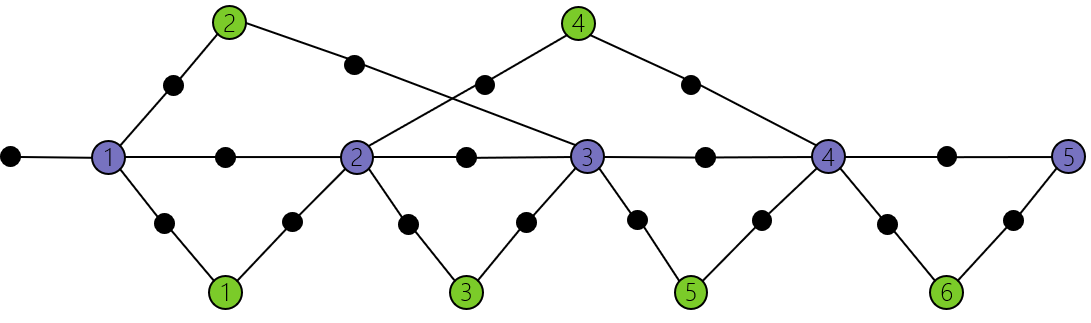
\includegraphics[scale=.7]{Pictures/factor_graph.png}
    \caption{因子图}
    \label{fig:factor_graph}
\end{figure}

如图~\ref{fig:factor_graph}是一个常见集束调整问题的因子图示例,其对应的正规方程具有如图~\ref{fig:normal_eq}所示的稀疏结构。按照式\eqref{eq:schur_complement}构建相机部分方程的舒尔补,依次迭代计算每一个三维点状态对应的舒尔补部分,并累加到图~\ref{fig:reduced_sys}中的高亮部分所示的舒尔补中。图~\ref{fig:schur_complement}展示了计算舒尔补的第一次迭代。

\begin{figure}[htb!]
    \centering
    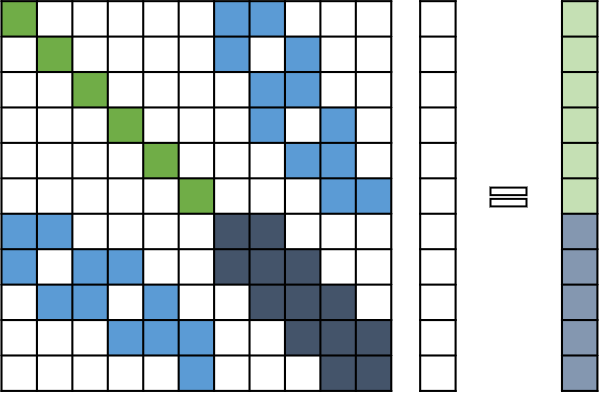
\includegraphics[scale=1]{Pictures/normal_eq.png}
    \caption{正规方程:左上角块对角矩阵部分对应三维点状态$1$至$6$的信息矩阵$\mathrm{P}$,右下角部分为相机状态$1$至$5$对应的信息矩阵$\mathrm{C}$,左下角和右上角为矩阵$\mathrm{W}$和$\mathrm{W}^\top$;中间列向量从上至下依次对应三维点状态$1$至$6$和相机状态$1$至$5$的迭代步;右侧部分从上至下依次对应三维点状态$1$至$6$和相机状态$1$至$5$。}
    \label{fig:normal_eq}
\end{figure}

\begin{figure}[htb!]
    \centering
    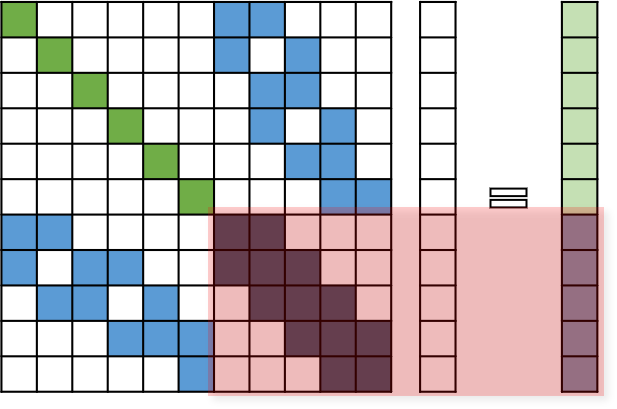
\includegraphics[scale=1]{Pictures/reduced_sys.png}
    \caption{舒尔补:高亮部分为相机状态对应舒尔补方程,其余部分为原方程。}
    \label{fig:reduced_sys}
\end{figure}

\begin{figure}[htb!]
    \centering
    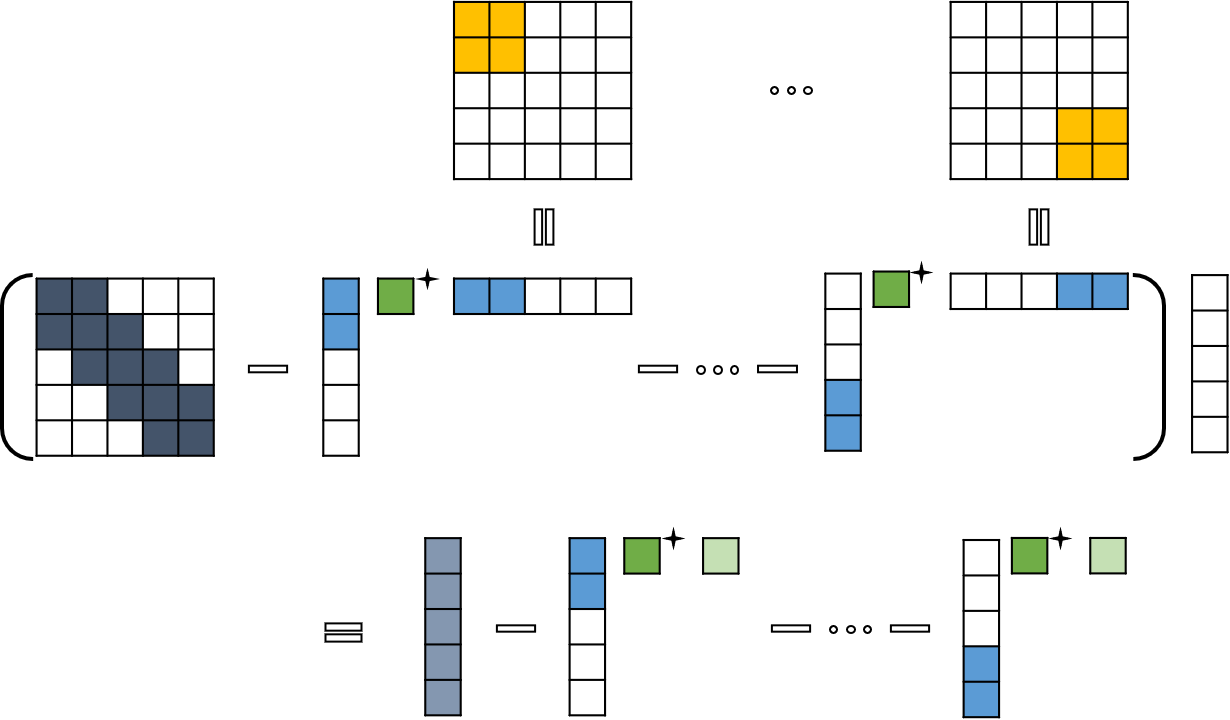
\includegraphics[width=\textwidth]{Pictures/schur_complement.png}
    \caption{计算舒尔补的一次迭代:从左上角开始依次迭代计算每一个三维点对应的舒尔补部分,并累加到右下角相机部分中。}
    \label{fig:schur_complement}
\end{figure}

\subsection{标记脏子图}

\begin{figure}[htb!]
    \centering
    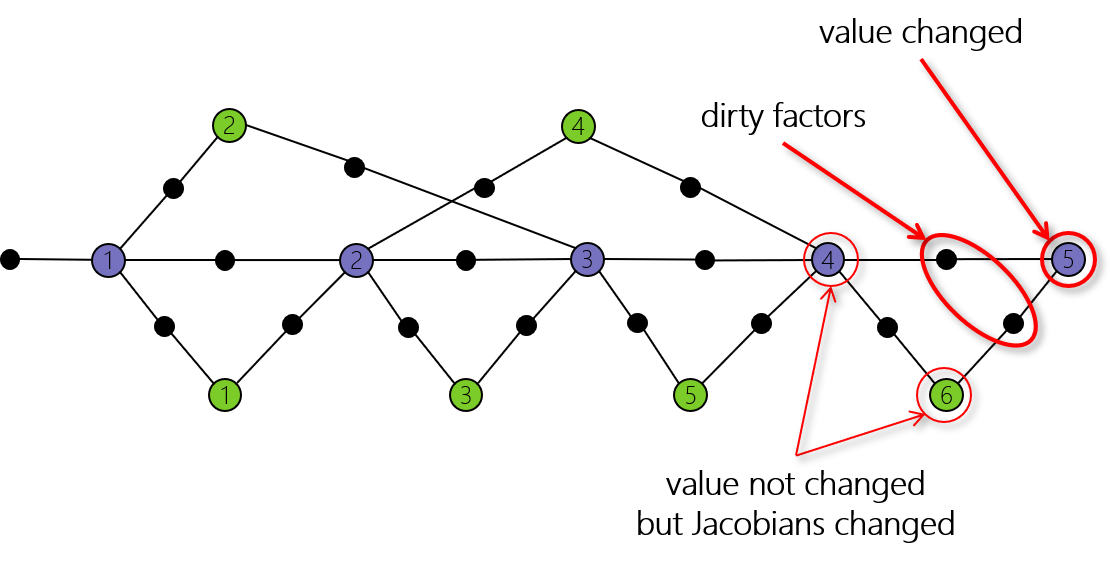
\includegraphics[scale=.7]{Pictures/factor_graph_dirty.png}
    \caption{因子图待更新部分:相机状态$5$为脏变量;与其直接相连的因子为脏因子;相机状态$4$和三维点状态$6$为只有梯度发生了变化的脏变量。这些节点构成了一个脏子图。}
    \label{fig:factor_graph_dirty}
\end{figure}

增量更新舒尔补的方法关键在于尽可能地复用上一次迭代的结果,只针对性地计算舒尔补方程中变化较大的变量对应的部分。以因子图~\ref{fig:factor_graph}为例,假设只有相机状态$5$有较大的更新,则先将其标记为脏变量。在因子图中,只有与脏变量直接相连的因子需要标记为脏因子,如图~\ref{fig:factor_graph_dirty}所示。需要注意的是,尽管相机状态$5$和三维点状态$6$的值并未发生足够大的改变,但是由于与之相连的部分因子被标记为脏因子,因此也需要更新这些因子关于它们的雅各比矩阵。这些脏变量和脏因子共同组成了一个脏子图,对应地,图~\ref{fig:normal_eq_dirty}高亮标示了舒尔补方程中需要更新的脏块。算法~\ref{alg:mark_dirty}详细说明了如何通过一个简单的宽度优先搜索标记出因子图中的脏子图。

\begin{algorithm}
\caption{标记脏子图}
\begin{algorithmic}
    \Require 因子图$\check{\mathcal{G}}=\{\check{\mathcal{F}},\check{\Theta},\check{\mathcal{E}}\}$,
             迭代步长$\bm{\delta}$
    \Ensure 脏子图$\mathcal{G}=\{\mathcal{F},\Theta,\mathcal{E}\}$

    \State $\mathcal{F}\coloneqq\{\}$,
           $\Theta\coloneqq\{\}$,
           $\mathcal{E}\coloneqq\{\}$

    \ForAll{$\left\|\bm{\delta}_i\right\| \geq \varepsilon$}
        \State $\Theta\coloneqq\Theta\cup\{\bm{\theta}_i\}$
        \Comment{将变量$\bm{\theta}_i$标记为脏变量}

        \ForAll
        {$\{
                \bm{f}_j\in\check{\mathcal{F}} |
                \bm{\theta}_i\in\Theta_j
        \}$}
        \Comment{$\Theta_j$为与$\bm{f}_j$相连的变量集合}
            \State $\Theta\coloneqq\Theta\cup\Theta_j$

            \State $\mathcal{E} \coloneqq \mathcal{E} \cup \{e_{ij}\}$
            \Comment{记录变量$\bm{\theta}_i$与因子$\bm{f}_j$相连的边$e_{ij}$}

            \State $\mathcal{F} \coloneqq \mathcal{F} \cup \{\bm{f}_j\}$
            \Comment{将因子$\bm{f}_j$标记为脏因子}
        \EndFor
    \EndFor
\end{algorithmic}
\label{alg:mark_dirty}
\end{algorithm}


\begin{figure}[htb!]
    \centering
    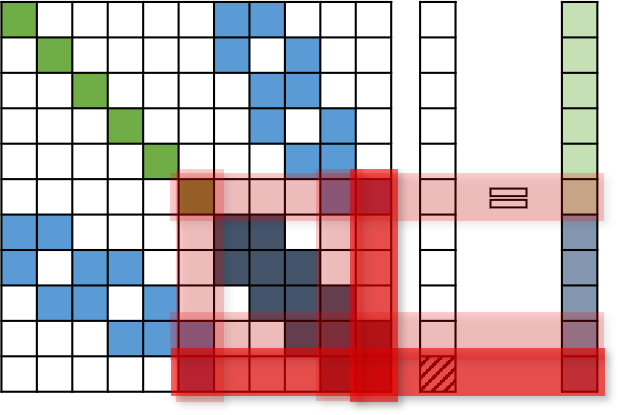
\includegraphics[scale=1]{Pictures/normal_eq_dirty.png}
    \caption{图~\ref{fig:factor_graph_dirty}对应的舒尔补方程中的脏块:相机状态$4$、$5$和三维点状态$6$构成的线性子系统。}
    \label{fig:normal_eq_dirty}
\end{figure}

\subsection{增量更新舒尔补}

舒尔补方程中被标记为脏块的矩阵构成了一个线性子系统,对应因子图中的脏子图。如图~\ref{fig:schur_update}所展示的,在增量更新舒尔补的过程中,需要先从舒尔补方程中减去脏子图的贡献,随后重新线性化所有的脏因子,最后重新计算舒尔补。算法~\ref{alg:schur_update}详细描述了这个过程。需要注意的是,在计算舒尔补的过程中会重复用到$\mathrm{W}_i\mathrm{P}_{ii}^{-1}\mathrm{W}_i^\top$,$\mathrm{W}_i\mathrm{P}_{ii}^{-1}\bm{p}_i$,$\mathrm{J}_j^\top\mathrm{J}_j$,$\mathrm{J}_j^\top\bm{f}_j$,需要将这些中间项缓存下来,避免重复计算。

\begin{algorithm}
\caption{增量更新舒尔补}
\begin{algorithmic}
    \Require 脏子图$\mathcal{G}=\{\mathcal{F},\Theta,\mathcal{E}\}$,
             上一轮迭代的$\bm{\delta}$,
             $\mathrm{H}$,$\bm{\eta}$,
             $\mathrm{S}$,$\bm{b}$
    \Ensure 更新后的
            $\mathrm{H}$,$\bm{\eta}$,
            $\mathrm{S}$,$\bm{b}$

    \ForAll{三维点状态$\bm{\theta}_i\in{\Theta}$}
    \Comment{减去三维点对舒尔补的贡献}
        \[\begin{aligned}
                \mathrm{S} &\coloneqq \mathrm{S} + \mathrm{W}_i{\mathrm{P}_{ii}}^{-1}\mathrm{W}_i^\top \\
                \bm{b}     &\coloneqq \bm{b}     + \mathrm{W}_i{\mathrm{P}_{ii}}^{-1}\bm{p}_i
        \end{aligned}\]
    \EndFor

    \ForAll{脏因子$\bm{f}_j\in\mathcal{F}$}
    \Comment{更新脏因子对正规方程的贡献}
        \[\begin{aligned}
                \mathrm{H} &\coloneqq \mathrm{H} - \mathrm{J}_j^\top \mathrm{J}_j \\
                \bm{\eta}  &\coloneqq \bm{\eta} + \mathrm{J}_j^\top \bm{f}_j
        \end{aligned}\]

        \[\begin{aligned}
                \mathrm{J}_j &\coloneqq \frac{\partial{\bm{f}_j(\Theta_j)}}
                                             {\partial{\Theta_j}} \\
                \bm{f}_j     &\coloneqq \bm{f}_j(\Theta_j)
        \end{aligned}\]

        \[\begin{aligned}
                \mathrm{H} &\coloneqq \mathrm{H} + \mathrm{J}_j^\top\mathrm{J}_j \\
                \bm{\eta}  &\coloneqq \bm{\eta}  - \mathrm{J}_j^\top\bm{f}_j
        \end{aligned}\]
    \EndFor

    \ForAll{三维点状态$\bm{\theta}_i\in{\Theta}$}
    \Comment{更新三维点对舒尔补的贡献}
        \[\begin{aligned}
                \mathrm{S} &\coloneqq \mathrm{S} - \mathrm{W}_i{\mathrm{P}_{ii}}^{-1}{\mathrm{W}_i}^\top \\
                \bm{b}     &\coloneqq \bm{b}     - \mathrm{W}_i{\mathrm{P}_{ii}}^{-1}\bm{p}_i
        \end{aligned}\]
    \EndFor

\end{algorithmic}
\label{alg:schur_update}
\end{algorithm}


\begin{figure}[htb!]
    \centering
    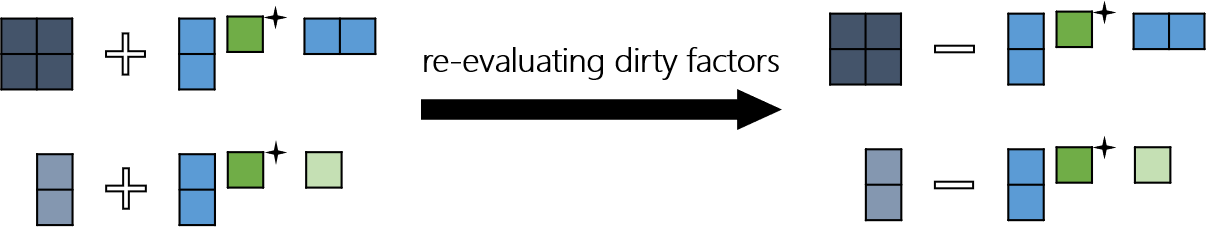
\includegraphics[width=\textwidth]{Pictures/schur_update.png}
    \caption{更新舒尔补}
    \label{fig:schur_update}
\end{figure}

\subsection{状态增广}

除了状态变量发生较大变化的时候需要更新因子图和舒尔补方程,集束调整过程中,如果有新的状态或因子加入,也需要对因子图进行增广,并对和舒尔补方程进行相应更新。实际上,这个过程也可以认为是算法~\ref{alg:schur_update}的一个特例。如图~\ref{fig:factor_graph_aug},新加入的状态通过新的因子与原因子图中相关联的部分状态共同构成了一个子图,将这个子图标记为脏子图,即可使用算法~\ref{alg:schur_update}进行更新。算法~\ref{alg:factor_graph_aug}给出了详细的过程,为了提高效率,因子图的增广和舒尔补方程的更新会被同时执行。

\begin{figure}[htb!]
    \centering
    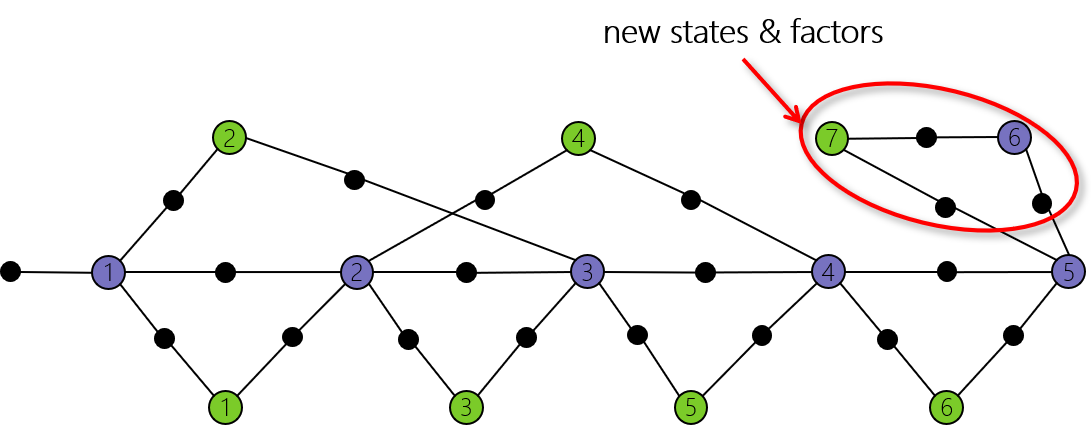
\includegraphics[scale=.7]{Pictures/factor_graph_aug.png}
    \caption{增广因子图}
    \label{fig:factor_graph_aug}
\end{figure}

\begin{figure}[htb!]
    \centering
    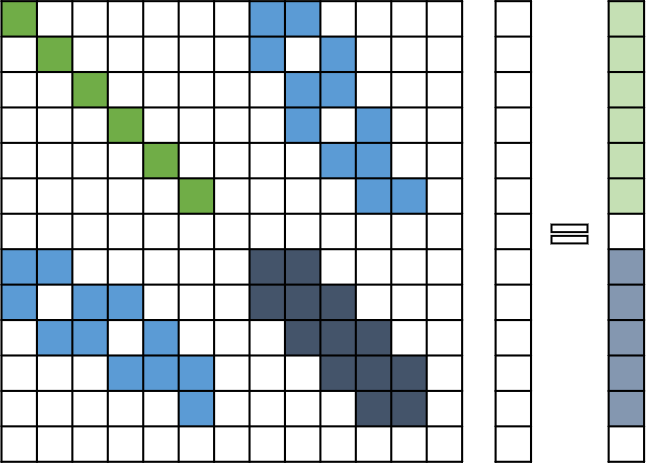
\includegraphics[scale=1]{Pictures/normal_eq_aug.png}
    \caption{增广正规方程}
    \label{fig:normal_eq_aug}
\end{figure}

\begin{figure}[htb!]
    \centering
    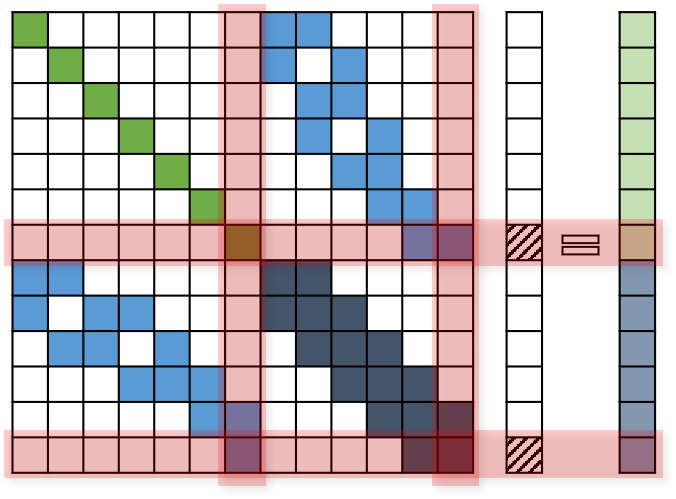
\includegraphics[scale=1]{Pictures/normal_eq_update.png}
    \caption{更新正规方程}
    \label{fig:normal_eq_update}
\end{figure}

\begin{algorithm}
\caption{状态增广}
\begin{algorithmic}
    \Require 因子图$\check{\mathcal{G}}=\{\check{\mathcal{F}},\check{\Theta},\check{\mathcal{E}}\}$,
             新加入的因子和状态$\{\mathcal{F}_0,\Theta_0\}$,
             上一次优化的
             $\mathrm{H}$,$\bm{\eta}$,
             $\mathrm{S}$,$\bm{b}$
    \Ensure 更新后的$\mathrm{H}$,$\bm{\eta}$,$\mathrm{S}$,$\bm{b}$

    \ForAll{三维点状态$\bm{\theta}_i\in{\Theta}_0$}
    \Comment{增广正规方程,如图~\ref{fig:normal_eq_aug}}
        \State 增广矩阵:$\mathrm{P}$,$\mathrm{W}$,$\bm{l}$
    \EndFor

    \ForAll{相机状态$\bm{\theta}_i\in{\Theta}_0$}
        \State 增广矩阵:$\mathrm{C}$,$\mathrm{S}$,$\mathrm{W}$,$\bm{c}$,$\bm{b}$
    \EndFor

    \State $\Theta\coloneqq\{\}$
    \Comment{更新正规方程和舒尔补,如图~\ref{fig:normal_eq_update}}

    \ForAll
    {$\{
            \bm{f}_j\in\mathcal{F}_0 |
            \Theta_j \cap \check{\Theta} \neq \emptyset
    \}$}
        \State $\Theta \coloneqq \Theta \cup (\Theta_j \cap \check{\Theta})$
    \EndFor

    \ForAll{三维点状态$\bm{\theta}_i\in{\Theta}$}
    \Comment{减去三维点对舒尔补的贡献}
        \[\begin{aligned}
                \mathrm{S} &\coloneqq \mathrm{S} + \mathrm{W}_i{\mathrm{P}_{ii}}^{-1}\mathrm{W}_i^\top \\
                \bm{b}     &\coloneqq \bm{b}     + \mathrm{W}_i{\mathrm{P}_{ii}}^{-1}\bm{l}_i
        \end{aligned}\]
    \EndFor

    \ForAll{脏因子$\bm{f}_j\in\mathcal{F}_0$}
        \Comment{更新新因子对正规方程的贡献}
        \[\begin{aligned}
                \mathrm{J}_j &\coloneqq \frac{\partial{\bm{f}_j}(\Theta_j)}
                                             {\partial{\Theta_j}} \\
                \bm{f}_j     &\coloneqq \bm{f}_j(\Theta_j)
        \end{aligned}\]

        \[\begin{aligned}
                \mathrm{H} &\coloneqq \mathrm{H} + \mathrm{J}_j^\top\mathrm{J}_j \\
                \bm{\eta}  &\coloneqq \bm{\eta}  - \mathrm{J}_j^\top\bm{f}_j
        \end{aligned}\]
    \EndFor

    \ForAll{三维点状态$\bm{\theta}_i\in{\Theta}$}
    \Comment{更新三维点对舒尔补的贡献}
        \[\begin{aligned}
                \mathrm{S} &\coloneqq \mathrm{S} - \mathrm{W}_i{\mathrm{P}_{ii}}^{-1}{\mathrm{W}_i}^\top \\
                \bm{b}     &\coloneqq \bm{b}     - \mathrm{W}_i{\mathrm{P}_{ii}}^{-1}\bm{l}_i
        \end{aligned}\]
    \EndFor

\end{algorithmic}
\label{alg:factor_graph_aug}
\end{algorithm}



\section{线性求解}\label{sec:lin_solver}

通过算法~\ref{alg:schur_update}更新舒尔补方程后,可以通过求解舒尔补方程快速得到相机状态的增量$\bm{\delta}_c$,再进一步通过回代求解三维点状态的增量$\bm{\delta}_l$。为了提升这部分求解数值稳定性,本文提出了使用混合式LM-DL方法(Hybrid Levenberg-Marquardt-Dog-Leg,简称HLMDL)求解舒尔补方程。在回代求解部分,受iSAM2\citep{kaess2012isam2}算法的启发,本文提出了使用部分贝叶斯推断树(Partial Bayes Tree,简称PBT)的方法编码三维点状态和相机状态之间的的推断关系,以达到增量式回代的目的,进一步提高效率。

\subsection{HLMDL方法求解舒尔补方程}

LM法的阻尼因子会影响正规矩阵的对角线元素,经过舒尔补操作之后,阻尼因子的影响被不可逆地累积到了舒尔补矩阵中,使得每次调整阻尼因子的时候必须要重新完整计算舒尔补。这会导致舒尔补无法进行增量更新,因此ICE-BA\citep{liu2018ice}和SLAM++中均使用DL法进行非线性求解。然而如第~\ref{ch:intro}~章中提到的,在实际求解线性问题时,往往会遇到矩阵秩亏或不正定的情况,而且这种情况在舒尔补矩阵中更为严重,这就造成了直接求解时数值不稳定的问题。为了避免这个问题,本文提出了改进,使用HLMDL的方法,在舒尔补矩阵的对角线上加上阻尼因子:
\begin{equation}
    \mathrm{S}' \doteq \mathrm{S}+\mu\mathbf{diag}(\mathrm{S})
\end{equation}
来改善舒尔补矩阵的秩亏现象。然后通过求解新的舒尔补方程得到相机状态增量$\bm{\delta}_c$:
\begin{equation}
    \bm{\delta}_c = \mathrm{S}' \:\setminus\: \bm{b}
    \label{eq:hlmdl}
\end{equation}
最后从$\mathrm{S}'$中减去阻尼因子的影响,恢复为原先的舒尔补矩阵:
\begin{equation}
    \mathrm{S} = \mathrm{S}'-\mu\mathbf{diag}(\mathrm{S})
\end{equation}
由于阻尼因子直接施加在构建好的舒尔补矩阵上而非原始的正规矩阵$\mathrm{H}$,其影响是可逆的,经过简单的操作即可恢复,在下一轮迭代中仍可以使用增量式方法更新舒尔补方程。通过HLMDL方法求得的$\bm{\delta}_c$是原始舒尔补方程的一个近似解,但是由于使用了迭代的方式求解,单次迭代的近似解对最终的结果影响很小。这里的阻尼因子的调整与DL的信赖信赖的调整是独立的,本文使用了\citen{tingleff2004methods}中的方法进行阻尼调节,逐步缩小阻尼因子,使得最后的解收敛于准确的解。

方程\eqref{eq:hlmdl}的求解可以使用任何常用的矩阵分解法,如QR分解、Cholesky分解等。也可以采用迭代式的线性求解方法,比如预处理共轭梯度法(preconditioned conjugate gradient,简称PCG)。本文提出的框架提供了自定义线性求解方法的接口,用户可以自己实现符合实际数值稳定性需求和求解效率要求的线性求解方法,也可以使用内置的Cholesky分解求解器和增量PCG(I-PCG)求解器。

由于HLMDL方法在舒尔补方程上施加了阻尼因子,本文没有使用增量式Cholesky分解\citep{polok2013incremental}来求解式\eqref{eq:hlmdl},而是提供了常规的Cholesky分解法和ICE-BA中提出的I-PCG方法,并配合Jacobi预处理方法\citep{jeong2012pushing}来提升线性求解的效率。

\subsection{使用PBT方法增量回代}

ICE-BA中使用了直接回代的方法求解三维点状态的增量,即求解完相机状态增量$\bm{\delta}_c$后,进一步使用式\eqref{eq:back_sub}直接批量回代求解三维点状态的增量$\bm{\delta}_l$。最后得到的总的状态增量$\bm{\delta}$,通过阈值判断其每个分量$\bm{\delta}_i$是否发生了足够大的更新并将发生较大更新的分量更新到状态中:
\begin{equation}
    \bm{x}_i \leftarrow \bm{x}_i + \bm{\delta}_i, \quad
    \forall \left\|\bm{\delta}_i\right\|_{\infty} \geq \varepsilon
\end{equation}

这一步求解并不是增量进行的,除了计算速度受到一定的影响,还存在变量更新不一致的问题。一种典型的情况是:某个相机状态$i$的增量$\bm{\delta}_i$较小,而与之相关的某个三维点状态$j$的增量$\bm{\delta}_{j}$发生了较大的更新,此时对应的因子$f(\bm{x}_i,\bm{x}_j)$被标记为脏因子,需要重新线性化$f(\bm{x}_i+\bm{\delta}_i,\bm{x}_j+\bm{\delta}_j)$,但由于$\bm{\delta}_i$较小而被忽略,实际计算的是$f(\bm{x}_i,\bm{x}_j+\bm{\delta}_j)$。这就造成变量更新的不一致,在实际运行过程中,会导致增量求解过程中能量收敛的变慢,影响求解效率。

针对这一情况,本文基于iSAM2算法的贝叶斯推断树方法提出了PBT方法,编码了三维点状态和相机状态之间的推断关系。iSAM2算法认为通过高斯消元法进行Cholesky分解或QR分解过程对应了将因子图转化为贝叶斯推断树的过程,贝叶斯推断树编码了所有变量之间的推断关系。在求解完根节点对应的变量之后,需要从根节点开始递归地回代求解叶节点。如果某个节点的变量的更新较小,则停止回代,其所有后代节点均不再继续回代求解(即使其中仍有可能有潜在的更新较大的节点)。这一操作使得整个回代求解过程与变量推断关系严格一致。

构建舒尔补的过程实际也是使用高斯消元将一部分变量(三维点状态)进行消去的过程,同样这个过程也可以生成贝叶斯推断树。以因子图~\ref{fig:factor_graph}为例,其舒尔补过程可以生成如图~\ref{fig:bayes_forest}所示的贝叶斯推断树。由于舒尔补只消去了三维点状态,而相机状态部分则保留原始状态,因此构建的贝叶斯推断树为部分贝叶斯推断树PBT,高度固定为$2$,所有相机变量共同构成了根节点,每一个叶节点代表一个三维点状态及其前置条件状态。

\begin{figure}[htb!]
    \centering
    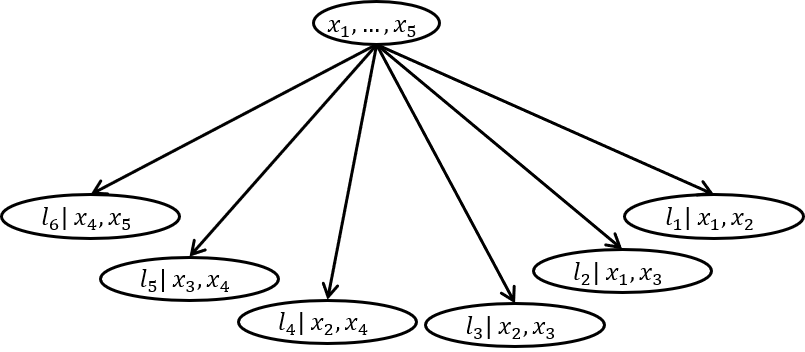
\includegraphics[scale=.8]{Pictures/bayes_forest.png}
    \caption{舒尔补构建的贝叶斯推断树}
    \label{fig:bayes_forest}
\end{figure}

利用PBT,可以方便地推断出任意一个三维点状态的前置条件变量。如果某个相机状态变量没有更新或更新较小,则以其为前置条件的三维点状态也不会更新(即使该三维点可能也发生了较大更新)。这就保证了三维点状态的更新和相机状态的更新的一致性。通过PBT回代求解得到$\bm{\delta}_l$后,进一步地,如果还需要进行下一轮迭代,则将综合更新量$\bm{\delta}$传递给算法~\ref{alg:mark_dirty},计算新一轮的迭代。整个增量舒尔补和线性求解的过程均可以基于块状稀疏矩阵实现。相比与稠密矩阵或一般的稀疏矩阵算法,块状稀疏矩阵的计算过程对cache更友好,也更适合使用CPU浮点指令集加速。得益于块状稀疏矩阵的高效,整个增量式集束调整的效率相比批量式集束调整可以有非常大的提升。


\section{增量式集束调整框架}

为了保证通用性,本文构建如图~\ref{fig:framework}所示的通用求解器的框架:

\begin{figure}[htb!]
    \centering
    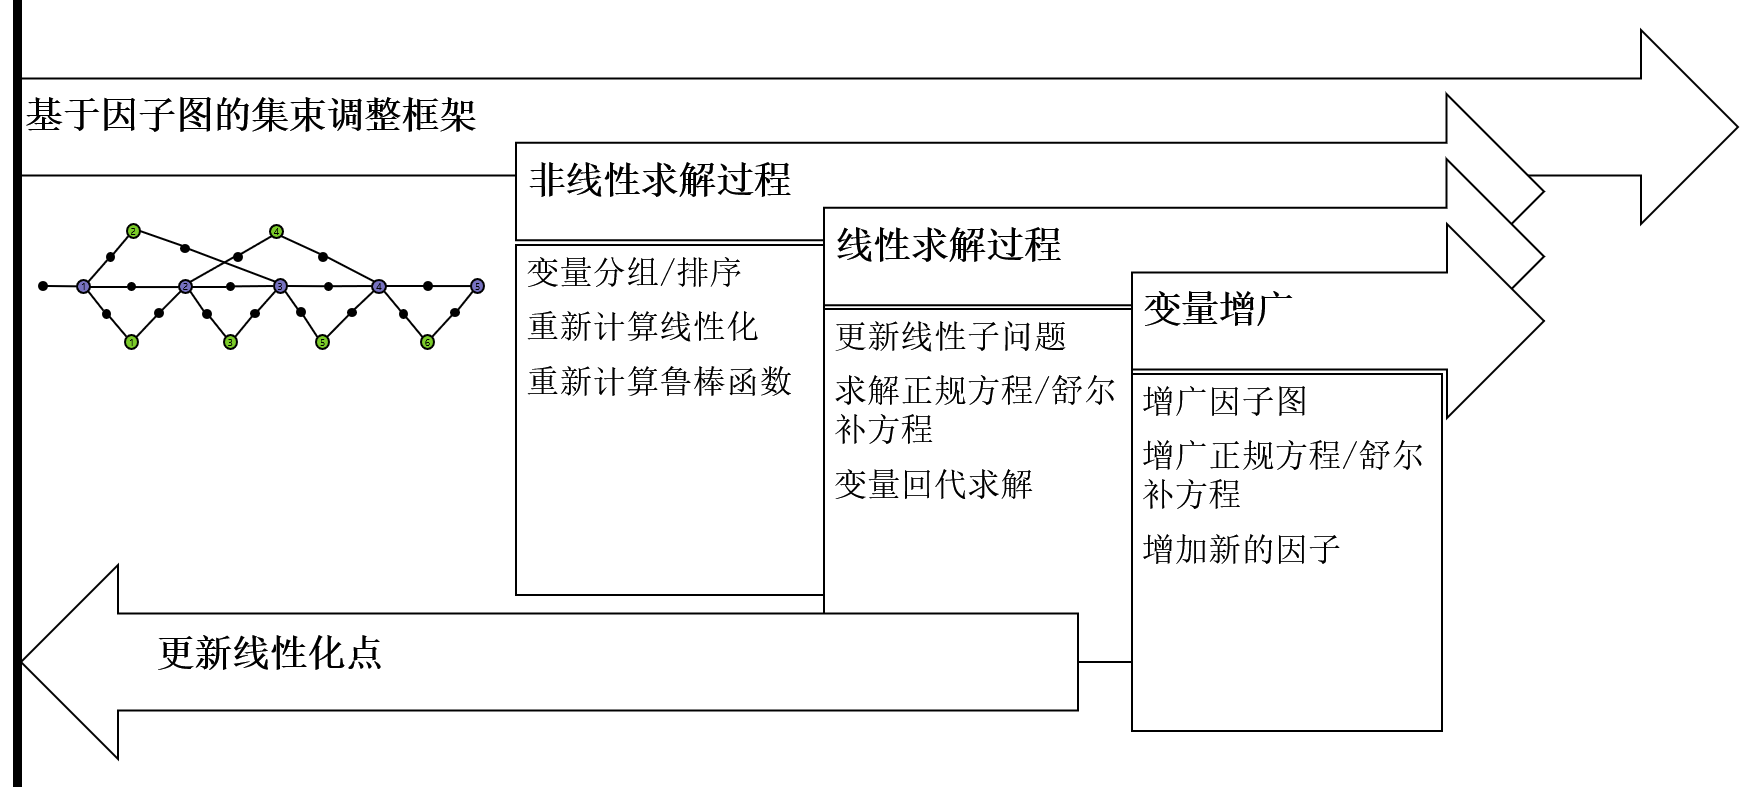
\includegraphics[scale=.5]{Pictures/framework.png}
    \caption{通用集束调整框架求解流程}
    \label{fig:framework}
\end{figure}

该框架的任意一个部分均可自定义实现,也可以采用内置的算法,具有很好的通用性和扩展性。表~\ref{tab:comp}展示了本文提出的增量式集束调整框架和其他增量式优化算法的对比

{
\linespread{1}
\begin{table}[H]
\zihao{6}
\caption{增量式集束优化求解器对比:加粗显示了不符合增量操作的部分}
\label{tab:comp}
\centering
\begin{tabular}{l|p{.2\textwidth} p{.2\textwidth} p{.2\textwidth} p{.2\textwidth}}
    \toprule
    求解器     & 本文提出的框架
               & ICE-BA
               & SLAM++
               & iSAM2
               \\ \midrule
    非线性部分 & a)三维点和相机状态分别成组
               & a)三维点和相机状态分别成组
               & a)三维点和相机状态分别成组
               & a)使用CCOLAMD对变量进行排序
               \\
               & b)根据构建舒尔补构建PBT
               &
               & b)相机部分使用COLAMD排序
               & b)通过消元构建贝叶斯树
               \\ \midrule
    线性化     & a)部分线性化
               & a)部分线性化
               & a)部分线性化
               & a)根据贝叶斯树进行即时线性化
               \\
               & b)根据脏子图增量更新舒尔补
               & b)根据脏变量更新舒尔补
               & b)根据脏变量更新舒尔补
               & b)更新平方根信息矩阵
               \\ \midrule
    线性求解   & a)\textbf{Cholesy分解或增量I-PCG求解舒尔补方程}
               & a)\textbf{I-PCG求解舒尔补方程}
               & a)\textbf{Cholesky分解求解舒尔补方程}
               & a)求解贝叶斯树根节点变量
               \\
               & b)根据PBT增量回代求解三维点
               & b)\textbf{完整回代求解三维点}
               & b)\textbf{完整回代求解三维点}
               & b)根据贝叶斯树增量回代求解剩余变量
               \\ \midrule
    变量更新   & 标记脏变量
               & 标记脏变量
               & 标记脏变量
               & 标记脏变量
               \\
    \bottomrule
\end{tabular}
\end{table}
}

需要注意的是,只有所有模块均符合增量操作的求解器才是完全增量的算法。而I-PCG仅仅是提高了收敛效率而没有降低时间复杂度,因此和Cholesky分解法一样,不属于增量操作。

\section{本章小结}

本章详细介绍了基于增量式舒尔补的集束调整优化算法,一组增量式集束调整优化的流程总结如下:
\begin{enumerate}
    \item 根据因子图,采用传统方法构建舒尔补并使用Cholesky分解或PCG方法求解首轮迭代,并构建PBT;
    \item\label{it:2} 使用算法~\ref{alg:mark_dirty}标记因子图和舒尔补方程需要更新的部分;
    \item\label{it:3} 使用算法~\ref{alg:schur_update}更新舒尔补;
    \item\label{it:4} 使用Cholesky分解或I-PCG方法求解舒尔补方程;
    \item\label{it:5} 基于PBT推断进行回代求解三维点状态;
    \item 重复步骤~\ref{it:2}至步骤~\ref{it:5}直到收敛;
    \item 当新增了因子或状态时,使用算法~\ref{alg:factor_graph_aug}进行增广,并重新从步骤~\ref{it:2}开始新一组优化
\end{enumerate}
